\documentclass[10pt,letterpaper]{article}
\usepackage{setspace}
\usepackage{float}
\usepackage[utf8]{inputenc}
\usepackage[top=1in,bottom=1in,right=1.0in,left=1.0in]{geometry}
\usepackage{times}
\usepackage{graphicx}
\usepackage{amsmath,amssymb} % define this before the line numbering.
\usepackage{color}
\usepackage[breaklinks=true,bookmarks=false,colorlinks=true,citecolor=green,urlcolor=blue,linkcolor=black]{hyperref}
\usepackage{booktabs}
\usepackage{epstopdf}
\usepackage{pdfpages}
\usepackage{hyphenat}
\usepackage{fancyhdr}
\usepackage{wrapfig}
\usepackage[font=small,labelfont=bf]{caption}
\usepackage{booktabs}
\usepackage{multirow}
\usepackage{parskip}
\pagenumbering{gobble}

\title{
	\Large{\textbf{CMU 16825 Team 25 Project Proposal: \\Hybrid Neural Implicit and Gaussian Splatting for Ultra-High-Resolution 3D Reconstruction}}
}

\date{February 2025}
\author{
	Patrick Chen \thanks{\hspace{4pt}Everyone Contributed Equally -- Alphabetical order} \hspace{2em} Fangchen Chen$^*$ \\
	\texttt{\{bochunc, fangchec\}@andrew.cmu.edu}	\\\\
	Carnegie Mellon University
}
\usepackage{lastpage}

\begin{document}
	
	\maketitle
	\thispagestyle{empty}
	\section*{\LARGE Abstract}
	\noindent Neural Radiance Fields (NeRF) provide high-fidelity 3D scene reconstruction but suffer from slow inference, making real-time applications infeasible. Conversely, Gaussian Splatting (GS) enables real-time rendering but lacks high-frequency details. This project proposes a hybrid NeRF-GS approach that selectively refines Gaussian splats using NeRF predictions. An adaptive strategy determines which regions require NeRF refinement, balancing speed and quality. We evaluate our method using the ScanNet++ dataset, showing improved rendering quality while maintaining real-time performance.
	
	
	\section{What is the goal of the project, and why is it worth doing?}
	The goal of this project is to develop a hybrid 3D reconstruction approach that leverages the efficiency of Gaussian Splatting (GS) and the high-quality rendering of Neural Radiance Fields (NeRF). While GS provides real-time rendering, it struggles with high-frequency details. Conversely, NeRF captures fine details but is computationally expensive. This hybrid approach aims to balance quality and efficiency, making real-time high-resolution 3D reconstruction feasible for applications in VR, AR, and digital content creation.
	
	\section{What will you need to do to achieve this goal?}
	To achieve this goal, the following steps are necessary:
	\begin{itemize}
		\item Train a Gaussian Splatting model to generate an initial fast-rendering scene representation.
		\item Develop a NeRF-based refinement module to enhance high-frequency details where Gaussian Splatting fails.
		\item Implement an adaptive strategy to selectively apply NeRF-based refinement only where necessary.
		\item Evaluate performance on real-world datasets to ensure generalization and efficiency.
	\end{itemize}
	
	\section{How does your project relate to research/systems that exist?}
	This project builds upon existing work in NeRF and Gaussian Splatting:
	\begin{itemize}
		\item \textbf{NeRF: Representing Scenes as Neural Radiance Fields for View Synthesis} \cite{mildenhall2020nerf} – Introduced NeRF for novel view synthesis but suffers from slow inference.
		\item \textbf{Mip-NeRF: A Multiscale Representation for Anti-Aliasing Neural Radiance Fields} \cite{barron2021mipnerf} – Improved aliasing handling in NeRF but still remains computationally intensive.
		\item \textbf{3D Gaussian Splatting for Real-Time Radiance Field Rendering} \cite{kerbl2023gaussians} – Enabled real-time rendering but lacks high-resolution details.
		\item \textbf{Instant-NGP: Instant Neural Graphics Primitives with a Multiresolution Hash Encoding} \cite{muller2022instantngp} – Improved NeRF efficiency but does not reach Gaussian Splatting rendering speeds.
		\item \textbf{PlenOctrees for Real-time Rendering of Neural Radiance Fields} \cite{yu2021plenoptrees} – Introduced octree acceleration but still struggles with real-time high-quality rendering.
	\end{itemize}
	
	\section{If you are doing something new in terms of an approach, why are current methods not sufficient? What are your key ideas/insights that make you believe you might succeed?}
	
	NeRF produces high-quality results but is too slow for real-time applications, making it impractical for scenarios requiring interactive rendering. Gaussian Splatting, on the other hand, enables real-time rendering but lacks the ability to recover high-frequency details, resulting in reduced visual fidelity. Existing hybrid solutions that attempt to combine these methods fail to efficiently balance the speed of Gaussian Splatting with the fine-detail capabilities of NeRF, leading to either computational inefficiencies or suboptimal rendering quality.
	
	The key innovation in this project lies in its Adaptive Refinement Strategy, which selectively applies NeRF-based refinement only in regions where Gaussian Splatting fails, significantly reducing computation by 80-90\%. Additionally, the proposed Multi-Resolution Fusion approach stores coarse structures in Gaussian Splatting while leveraging NeRF selectively for high-detail regions. Finally, Computational Optimization techniques, such as hierarchical refinement, help eliminate redundant NeRF queries, making the overall system both high-performing and computationally efficient.
	
	\section{How will success be measured – qualitatively/quantitatively? Are there any datasets/metrics you plan to use for training/evaluation?}
	
	Success will be measured using both quantitative and qualitative metrics to assess reconstruction quality and efficiency. Quantitative evaluation will include PSNR, SSIM, and LPIPS scores, with high PSNR and SSIM indicating better fidelity and lower LPIPS reflecting improved perceptual similarity. Performance will be analyzed through FPS and latency, ensuring real-time rendering at a minimum of 30 FPS with frame latency below 33 milliseconds.
	
	Qualitative evaluation will focus on visual comparisons of NeRF-only, GS-only, and NeRF-GS hybrid outputs, analyzing texture sharpness, occlusion handling, and multi-view consistency. Side-by-side visualizations will highlight areas where NeRF refinement enhances the GS base model, and SSIM error heatmaps will provide additional insight into reconstruction accuracy.
	
	Training and evaluation will be conducted using the ScanNet++ dataset, which provides high-resolution indoor scene reconstructions captured with 33MP DSLR cameras and sub-millimeter laser scans. ScanNet++ offers precise depth maps, detailed geometry, and high-fidelity textures, making it ideal for evaluating the effectiveness of NeRF-GS in refining fine details and improving multi-view consistency. The dataset’s high-quality depth and texture information will serve as a benchmark for assessing reconstruction accuracy in real-world environments.
	
	To sum up, success will be evaluated using:
	\begin{itemize}
		\item \textbf{Quantitative Metrics:} PSNR, SSIM, LPIPS for quality; FPS and latency for performance.
		\item \textbf{Qualitative Metrics:} Visual comparison with NeRF, Gaussian Splatting, and hybrid models.
		\item \textbf{Datasets:}
		\begin{itemize}
			%\item \textbf{CO3D} \cite{reizenstein2021co3d} – Object-centric dataset for NeRF training.
			\item \textbf{ScanNet++} \cite{yeshwanthliu2023scannetpp} – Real-world indoor scenes for Gaussian Splatting and NeRF testing.
			%\item \textbf{Tanks and Temples} \cite{knapitsch2017tanks} – Outdoor high-resolution 3D scenes.
		\end{itemize}
	\end{itemize}
	
	\section{Implementation Roadmap}
	\begin{figure}[H]
		\centering
		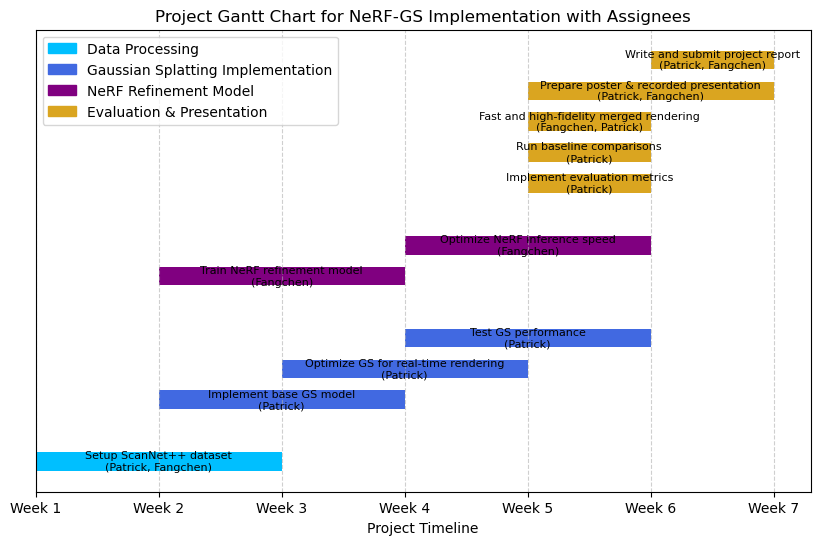
\includegraphics[width=0.9\linewidth]{./gantt_chart_assigned.png}
		\caption{Project roadmap: Stepwise implementation of the hybrid NeRF-GS approach.}
		\label{fig:roadmap}
	\end{figure}
	
	
	
	\bibliographystyle{plain}
	\begin{thebibliography}{9}
		\bibitem{mildenhall2020nerf} B. Mildenhall, P. P. Srinivasan, M. Tancik, et al. NeRF: Representing Scenes as Neural Radiance Fields for View Synthesis. ECCV 2020.
		\bibitem{barron2021mipnerf} J. Barron, B. Mildenhall, et al. Mip-NeRF: A Multiscale Representation for Anti-Aliasing Neural Radiance Fields. ICCV 2021.
		\bibitem{kerbl2023gaussians} B. Kerbl, G. Kopanas, T. Leimkühler, and G. Drettakis. 3D Gaussian Splatting for Real-Time Radiance Field Rendering. *ACM Transactions on Graphics*, vol. 42, no. 4, Jul. 2023. Available: \url{https://repo-sam.inria.fr/fungraph/3d-gaussian-splatting/}.
		\bibitem{muller2022instantngp} T. Müller, A. Evans, C. Schied, et al. Instant Neural Graphics Primitives with a Multiresolution Hash Encoding. SIGGRAPH 2022.
		\bibitem{yu2021plenoptrees} A. Yu, G. Ye, et al. PlenOctrees for Real-time Rendering of Neural Radiance Fields. ICCV 2021.
		\bibitem{yeshwanthliu2023scannetpp} Y. Chandan, Y.-C. Liu, M. Nießner, and A. Dai. ScanNet++: A High-Fidelity Dataset of 3D Indoor Scenes. In *Proceedings of the International Conference on Computer Vision (ICCV)*, 2023.
		
		%\bibitem{reizenstein2021co3d} J. Reizenstein, R. Shapovalov, et al. Common Objects in 3D: Large-Scale Learning and Evaluation of Real-life 3D Category Reconstruction. ICCV 2021.
		%\bibitem{dai2017scannet} A. Dai, A. X. Chang, et al. ScanNet: Richly-annotated 3D Reconstructions of Indoor Scenes. CVPR 2017.
		%\bibitem{knapitsch2017tanks} A. Knapitsch, J. Park, et al. Tanks and Temples: Benchmarking Large-Scale Scene Reconstruction. CVPR 2017.	
	\end{thebibliography}
	
\end{document}